% capitulo1.tex
\chapter{Introducción}

\section{Problema 16 de Hilbert}
En 1900, el matemático alemán David Hilbert presentó una lista de 23 problemas abiertos en el Congreso Internacional de Matemáticos en París. Estos problemas de diversas áreas de las matemáticas, se convirtieron en una guía fundamental para la investigación matemática del siglo XX y, en muchos casos, aún siguen desafiando a la comunidad científica. \cite{hilbert1902mathematical}

El \textbf{problema 16 de Hilbert} forma parte de esta lista y está dividido en dos partes principales. Ambas se centran en el análisis geométrico y topológico de curvas algebraicas y sistemas dinámicos polinomiales en el plano:

\begin{enumerate}
	\item \textbf{Primera parte:} Clasificar las disposiciones topológicas posibles de las curvas algebraicas planas reales de grado $n$. Este problema está relacionado con la geometría algebraica real y la topología.
	\item \textbf{Segunda parte:} Estudiar los sistemas dinámicos definidos por campos vectoriales polinomiales en el plano, y en particular, determinar el número máximo y la disposición de los ciclos límite que estos sistemas pueden tener.
\end{enumerate}

La segunda parte del problema 16 de Hilbert aborda una cuestión fundamental en la teoría de sistemas dinámicos: la existencia, finitud y disposición de ciclos límite en sistemas de ecuaciones diferenciales polinomiales. Un ciclo límite es una órbita cerrada aislada en el espacio de fases, alrededor de la cual las trayectorias vecinas convergen o divergen en espiral hacia adentro o hacia afuera. 

Los ciclos límite son fundamentales en la teoría de sistemas dinámicos porque representan comportamientos oscilatorios estables o inestables, aunque formulado hace más de un siglo, el problema 16 de Hilbert sigue siendo relevante hoy en día debido a sus aplicaciones en biología, ingeniería y física, donde los ciclos límite modelan fenómenos oscilatorios fundamentales \cite{ilyashenko2002centennial}.

Consideremos el sistema de ecuaciones en el plano polinomial de grado $n$:

\begin{equation}
	x'=P\left(x,y\right)\text{, }\text{  }y'=Q\left(x,y\right)
\end{equation}
donde $P\left(x,y\right)$ y $Q\left(x,y\right)$ son polinomios de grado a lo más $n$, por lo que son funciones suaves. El problema consiste en responder las siguientes preguntas:
\begin{enumerate}
	\item ¿Cuántos ciclos límite puede tener un sistema polinómico de grado $n$?
	\item ¿Cómo están distribuidos estos ciclos límite en el plano?
\end{enumerate}

¿Sencillo? pues no, la respuesta sigue siendo desconocida para $n>1$, a mayor grado, mayor complejidad del sistema y la estructura de sus soluciones. La dificultad radica en la naturaleza no lineal de los sistemas dinámicos y en la interacción entre las singularidades y las órbitas cerradas.

\section{Resultados relevantes sobre la existencia de ciclos límite}

Tenemos algunos resultados significativos como la conjetura de Dulac, que establece que para cualquier $n$, el número de ciclos límite de un sistema polinómico de grado $n$ es finito, sin embargo esto es una conjetura y aún no se ha probado. Analicemos los resultados más relevantes conocidos hasta la fecha acerca de la existencia de ciclos límite en el contexto del problema 16 de Hilbert.

\begin{enumerate}
	\item \textbf{Teorema de Poincaré-Bendixson} Establece las condiciones suficientes para la existencia de ciclos límite en sistemas planares. En el siguiente capítulo vamos a desarrollar este teorema y su demostración \cite{perko2001differential}.
	
	\item \textbf{Conjetura de Finitud de Dulac}\\

	Este resultado es crucial porque establece un marco teórico para acotar el número de ciclos límite en sistemas polinomiales, aunque el valor exacto sigue siendo desconocido.
	\begin{itemize}
		\item En 1923, Henri Dulac planteó la conjetura de que el número de ciclos límite de un sistema polinómico de grado $n$ en el plano es finito \cite{dulac1923cycles}.
		\item Jean Écalle y Yulij Il'yashenko, de forma independiente en 1991, probaron la conjetura de finitud de Dulac. Demostraron que para sistemas polinómicos planos, el número de ciclos límite es finito. Este resultado es significativo porque confirma que, aunque no se conoce el número máximo exacto de ciclos límite para cada grado $n$, al menos se sabe que este número es finito \cite{ecalle1992correction, ilyashenko1991finiteness}.
	\end{itemize}

	\item \textbf{Sistemas Polinomiales de Bajo Grado}
	\begin{itemize}
		\item Los sistemas lineales en el plano ($n=1$) no poseen ciclos límite. Toda órbita es o bien una trayectoria hacia o desde un punto de equilibrio, o una familia de órbitas paralelas.

		\item Hasta ahora, el máximo número de ciclos límite conocidos en sistemas cuadráticos es $4$, pero no se ha probado que este sea el número máximo posible. Nikolai Bautin en 1939 analizó las bifurcaciones en sistemas cuadráticos y encontró condiciones para la aparición de ciclos límite pequeños alrededor de puntos singulares.
	\end{itemize}

	\item \textbf{Teoría de Bifurcaciones y Ciclos Límite}
	La teoría de bifurcaciones ha sido una herramienta clave en el estudio de los ciclos límite.
	\begin{itemize}
		\item \textbf{Bifurcación de Hopf}: Describe cómo un ciclo límite puede emerger o desaparecer al variar un parámetro en el sistema.
		\item \textbf{Ciclos Límite Múltiples}: Investigaciones han mostrado que es posible tener múltiples ciclos límite que rodean puntos singulares o áreas sin puntos singulares.
	\end{itemize}
	\item \textbf{Métodos Analíticos y Geométricos}
	\begin{itemize}
		\item \textbf{Función de Dulac}
		Dulac introdujo una función auxiliar (ahora conocida como función de Dulac) para estudiar la no existencia de ciclos límite en ciertas regiones. Este resultado es crucial porque establece un marco teórico para acotar el número de ciclos límite en sistemas polinomiales, aunque el valor exacto sigue siendo desconocido.
		\item \textbf{Teoría de Hilbert-Poincaré}
		Variedades Algebraicas: Se utilizan herramientas de geometría algebraica para entender las propiedades globales de los sistemas polinómicos.
		
		\item \textbf{Análisis de Singularidades}: El estudio de puntos críticos y sus tipos es esencial para comprender la dinámica local y global.
	\end{itemize}

	\item \textbf{Métodos de Perturbación}
	Se han utilizado métodos de perturbación y teoría de promediación para estudiar la aparición de ciclos límite en sistemas cercanos a sistemas integrables.
	\item \textbf{Teoría de Foliaciones}
	El estudio de foliaciones en el plano ha proporcionado nuevas perspectivas sobre la estructura de las órbitas y la posible existencia de ciclos límite.
\end{enumerate}

\section{Problemas clásicos de ciclos límite}

Los sistemas dinámicos ofrecen la posibilidad de explorar comportamientos oscilatorios que son inherentes a muchos procesos biológicos, químicos y físicos. A continuación, se presentan varios ejemplos donde los ciclos límite desempeñan un papel central.

\begin{itemize}
	\item \textbf{Oscilador de Van der Pol}\\

	El oscilador de Van der Pol es un ejemplo clásico de un sistema no lineal que exhibe ciclos límite. Originalmente desarrollado para modelar circuitos eléctricos con tubos de vacío, este sistema también describe fenómenos auto-oscilatorios en ingeniería y biología \cite{vanderpol1926forced}.
	\begin{equation}
		x''-\mu \left(1-x^2\right)x'+x=0
	\end{equation}
	donde $\mu$ es el coeficiente de amortiguamiento. A medida que $\mu$ aumenta, el sistema muestra un ciclo límite estable que corresponde a una oscilación sostenida. Este comportamiento es crucial para entender dispositivos electrónicos oscilatorios y ciertos ritmos biológicos.

	\begin{figure}[h]
		\centering
		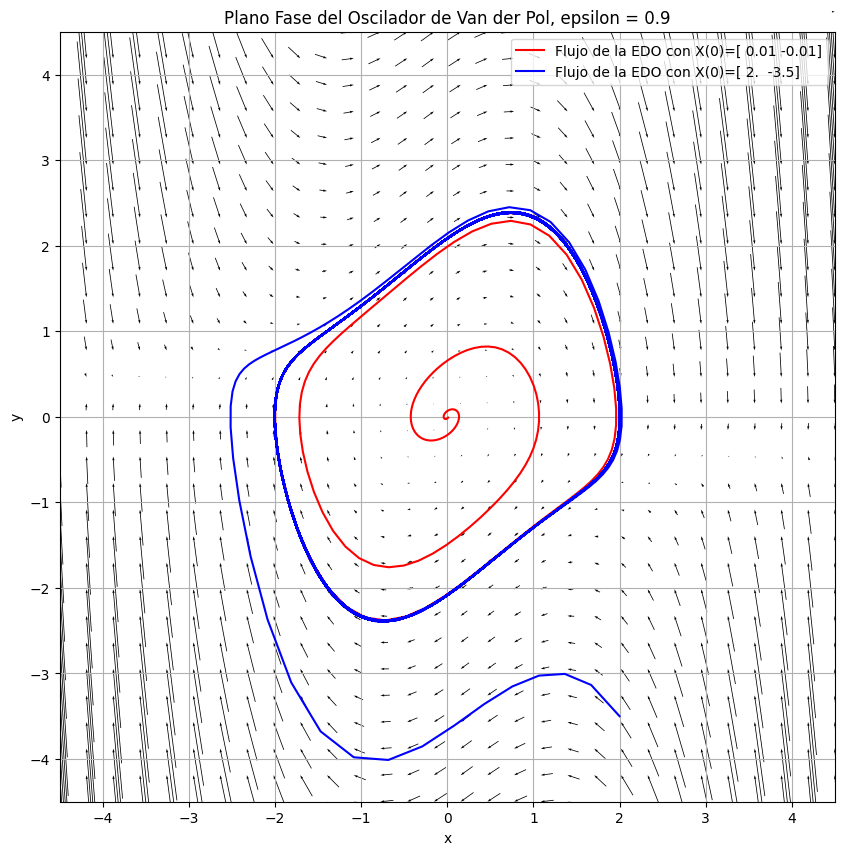
\includegraphics[width=11cm]{introVanderPol.png}
		\caption{Plano fase del Oscilador de Van der Pol}
        \label{fig:introVanderPol}
	\end{figure}

	El oscilador de Van der Pol es un caso particular de un sistema polinomial de grado 2 (del Problema 16° de Hilbert), y su estudio proporciona intuiciones sobre la existencia y distribución de ciclos límite en sistemas más generales.

	\newpage

	\item \textbf{Ecuación de Rayleigh}\\

	La ecuación de Rayleigh modela el comportamiento de ciertos sistemas mecánicos y fluidos sometidos a fuerzas periódicas. Es similar al oscilador de Van der Pol \cite{rayleigh1883theory}.
	\begin{equation}
		x''+x=\epsilon\left(1-x'^2\right)x'
	\end{equation}
	donde $\epsilon$ controla la intensidad de la fuerza. Los ciclos límite en este modelo describen el fenómeno de resonancia mecánica y son fundamentales para el diseño de sistemas que requieren estabilidad en las oscilaciones, como los amortiguadores en vehículos.

	\begin{figure}[h]
		\centering
		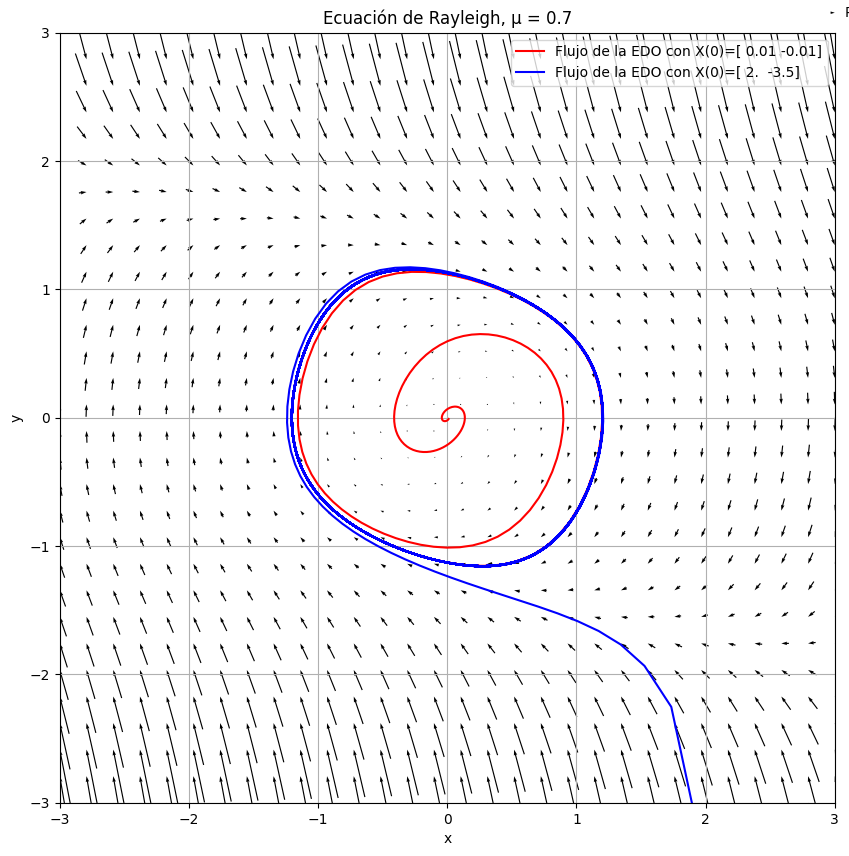
\includegraphics[width=13cm]{introRayleigh.png}
		\caption{Plano fase de la ecuación de Rayleigh}
        \label{fig:introRayleigh}
	\end{figure}

	\newpage

	\item \textbf{Modelo de Fitz Hugh-Nagumo}\\

	Este modelo es una simplificación del modelo de Hodgkin-Huxley y se utiliza para describir la activación y desactivación de las neuronas \cite{fitzhugh1961impulses, nagumo1962active}.
	\begin{equation}
		\begin{matrix}
			v'=v-\frac{v^3}{3}-w+I\\
			w'=\epsilon\left(v+a-bw\right)
		\end{matrix}
	\end{equation}
	donde $v$ representa el potencial de membrana, $w$ es una variable de recuperación, e $I$ es un término de corriente externa. Los ciclos límite en este sistema modelan los potenciales de acción neuronal, esenciales para entender el procesamiento de la información en el cerebro.

	\begin{figure}[h]
		\centering
		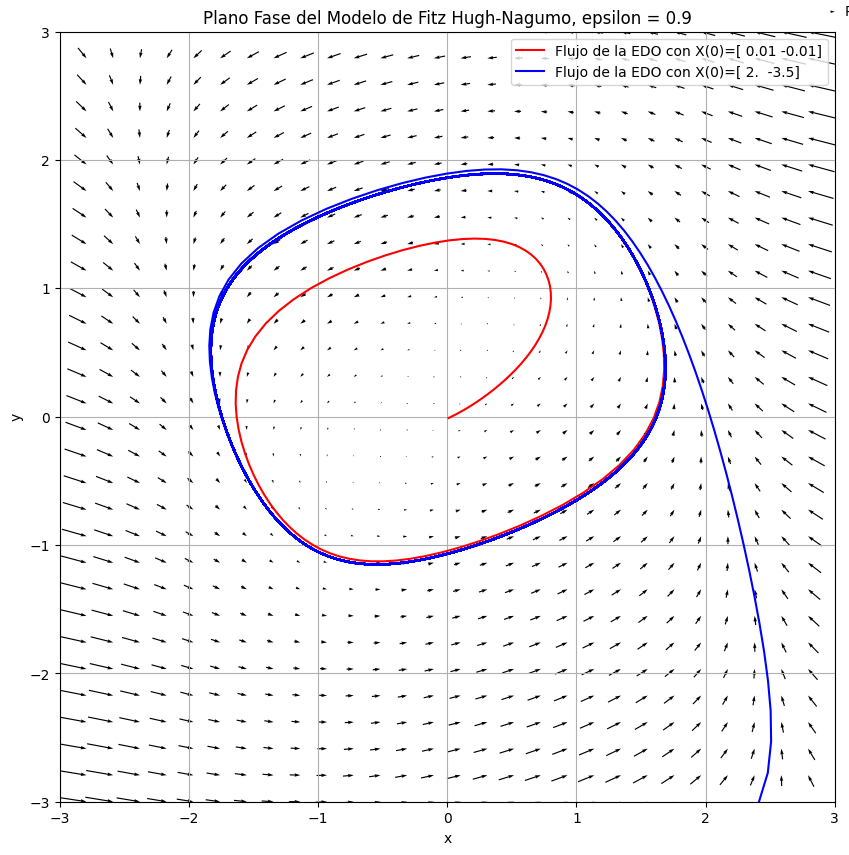
\includegraphics[width=12cm]{introFitz.png}
		\caption{Plano fase del Modelo de Fitz Hugh-Nagumo}
        \label{fig:introFitz}
	\end{figure}

	\newpage

	\item \textbf{Reacciones Químicas Oscilatorias}\\

	Un ejemplo destacado es la reacción de Belousov-Zhabotinsky, que es un tipo de reacción química que muestra oscilaciones temporales en la concentración de sus reactivos. Aunque su modelado exacto requiere ecuaciones más complejas, sistemas simplificados que muestran ciclos límite pueden ayudar a comprender la dinámica subyacente de estas reacciones oscilatorias \cite{zhabotinsky1964periodic}.
\end{itemize}
Más adelante vamos a desarrollar estos modelos a profundidad.

\section{Aplicaciones modernas de los ciclos límite}

El estudio de los ciclos límite tiene una amplia gama de aplicaciones en diversas disciplinas científicas e ingenieriles, destacando su relevancia tanto en contextos teóricos como prácticos. Estas son algunas de las áreas más significativas donde los ciclos límite han demostrado ser herramientas fundamentales para modelar y comprender fenómenos oscilatorios y dinámicos.

\begin{enumerate}
	\item \textbf{Biología y Medicina}\\

	En biología, los ciclos límite son esenciales para describir sistemas dinámicos que exhiben comportamientos periódicos o cuasiperiódicos. En fisiología, los ciclos límite permiten modelar ritmos circadianos, regulando procesos biológicos como el ciclo sueño-vigilia y el metabolismo. En neurociencia, estos conceptos explican patrones oscilatorios en redes neuronales, incluyendo potenciales de acción y trastornos como la epilepsia o el Parkinson. Además, en cardiología, los ciclos límite ayudan a analizar arritmias cardíacas y otros fenómenos oscilatorios en el sistema cardiovascular \cite{murray2002mathematical}.
	\item \textbf{Ingeniería}\\

	En ingeniería, los ciclos límite encuentran aplicaciones en sistemas no lineales que requieren control preciso y estabilidad. Por ejemplo, en electrónica, los osciladores de Van der Pol son fundamentales para generar señales periódicas utilizadas en telecomunicaciones y relojes digitales. En robótica, los ciclos límite modelan comportamientos cíclicos, como caminar, nadar o volar, permitiendo el diseño de robots autónomos con movimientos eficientes. En el ámbito aeroespacial, estos conceptos son útiles para analizar vibraciones autoinducidas en turbinas o alas de aviones, así como para diseñar mecanismos de control de vuelo. También en energías renovables, los ciclos límite contribuyen a la estabilidad de redes eléctricas con fuentes intermitentes, como la sincronización de inversores solares \cite{khalil2002nonlinear}.
	\item \textbf{Física, Química y Clima}\\

	En física, los ciclos límite describen fenómenos oscilatorios en sistemas mecánicos no lineales, como péndulos forzados o sistemas con fricción. En óptica no lineal, estos conceptos modelan oscilaciones en la intensidad de luz emitida por láseres, mientras que en dinámica de fluidos, representan estados oscilatorios estables en flujos turbulentos o caóticos. En ciencias del clima, los ciclos límite son útiles para estudiar sistemas como El Niño y La Niña, que exhiben oscilaciones cuasiperiódicas. Además, en plasmas y fusión nuclear, modelos basados en ciclos límite describen el transporte de partículas y energía en reactores como los Tokamak \cite{guckenheimer1983nonlinear}.
	\item \textbf{Economía y Ciencias Sociales}\\

	En economía, los ciclos límite proporcionan una base para modelar fluctuaciones cíclicas en variables macroeconómicas, como el ciclo económico de expansión y recesión. En ciencias sociales, estos conceptos se aplican al análisis de dinámicas colectivas, como la propagación de enfermedades o la evolución de opiniones públicas en redes sociales. Los ciclos límite también son relevantes en el estudio de sistemas complejos, donde patrones recurrentes de comportamiento emergen de interacciones locales \cite{wiggins2003introduction}.
\end{enumerate}

Vamos a desarrollar algunos de estas aplicaciones en capítulos posteriores, pero antes, vamos a desarrollar la teoría de los ciclos límite en un contexto más general.
En los siguientes capítulos, utilizaremos herramientas como el teorema de Poincaré-Bendixson y métodos de promediación para analizar la existencia y distribución de ciclos límite en sistemas polinomiales de grado $n$, contribuyendo así a resolver aspectos abiertos del problema 16 de Hilbert.
